%%%%%%%%%%%%%%%%%%%%%%%%%%%%%%%%%%%%%%%%%%%%%%%%%%%%%%%%%%%%%%%%%
%
% Project     : Bachelorarbeit
% Title       : Machbarkeitsanalyse für eine ressourcenorientierte Schnittstelle zur Verarbeitung grundlegender Probleme der Informatik
% File        : einleitung.tex Rev. 01
% Date        : 01.03.2015
% Author      : Raffael Santschi
%
%%%%%%%%%%%%%%%%%%%%%%%%%%%%%%%%%%%%%%%%%%%%%%%%%%%%%%%%%%%%%%%%%

\chapter{Theoretische Grundlagen}\label{chap.einleitung}
Die theoretischen Grundlagen dienen dazu, wichtige Informationen zum Verständnis der Arbeit zu erläutern. Es werden die Komplexitätsklassen der theoretischen Informatik und die verschiedenen 
Algorithmentypen erklärt.

\section{Komplexitätsklassen der theoretischen Informatik}\label{cat_theo_inf}
In der theoretischen Informatik wird zwischen verschiedenen Komplexitätsklassen unterschieden. In diesem Kapitel wird nur auf die Komplexitätsklassen \gls{np}, \gls{p}, \gls{np}-schwer und 
\gls{np}-vollständig eingegangen, weitere Klassen wie zum Beispiel Random Polynomial (RP) oder Zero-Error Probabilistic Polynomial (ZPP) werden nicht erläutert, da sie nicht für das Verständnis der 
Arbeit notwendig sind. Die nachfolgenden Erklärungen sind aus \cite{hopcroft2011einfuehrung} und \cite{slides_p_np} abgeleitet.

\subsection{P}\label{p_complet}
Probleme, welche in \gls{polynomialzeit} mit Hilfe einer \glslink{deterministisch}{deterministischen} \gls{turingmaschine} lösbar sind, gehören zu der Klasse der \gls{p} Probleme. In 
\gls{polynomialzeit} lösbar heisst, dass die Laufzeitkomplexität in einem Polynom mit der Form $n^k$ dargestellt werden kann, wobei n die Eingabelänge und k eine Konstante ist.

\subsection{NP}\label{np}
\gls{np} Probleme können mit Hilfe einer \glslink{nichtdeterministisch}{nichtdeterministischen} \gls{turingmaschine} in \gls{polynomialzeit} gelöst werden. Zusätzlich muss die Korrektheit einer 
Lösung zu einem \gls{np} Problem ebenfalls in \gls{polynomialzeit} überprüft werden können. Die Prozedur, welche für die Überprüfung benötigt wird, wird \gls{polynomialzeit_verifizierer} 
genannt.

\subsection{NP-schwer}\label{np_hard}
Um zu beweisen, dass ein Problem \gls{np}-schwer ist, müssen für alle bekannten \gls{np}-schweren Probleme eine \gls{polynomialzeitreduktion} auf dieses Problem durchgeführt werden können. 
Mit diesem Beweis wird gezeigt, dass das Problem mindestens so schwer wie die anderen Probleme ist. Stephen Cook hat die \gls{np}-Schwere des SAT-Problems bewiesen, indem er die 
Arbeitsweise einer \glslink{nichtdeterministisch}{nichtdeterministischen} \gls{turingmaschine} durch eine logische Formel beschrieb \cite{cook_complexity}. Wenn das SAT-Problem gelöst 
werden kann, kann auch entschieden werden, ob die \glslink{nichtdeterministisch}{nichtdeterministische} \gls{turingmaschine} hält, somit ist SAT \gls{np}-schwer. Die derzeit bekannten 
Algorithmen zur Lösung \gls{np}-schwerer Probleme besitzen eine Laufzeitkomplexität höher als polynomial, zum Beispiel $k^n$ (exponentiell) oder $n!$ (faktoriell). Die Probleme werden in 
Entscheidungsprobleme und Optimierungsprobleme, bei welche die optimale Lösung gesucht wird, unterteilt.

\subsection{NP-vollständig}\label{np_complet}
Stephen Cook bewies nicht nur die \gls{np}-Schwere des SAT-Problems. Er zeigte auch, dass die Überprüfung einer Lösung in \gls{polynomialzeit} möglich ist. Das SAT-Problem ist somit
\gls{np}-vollständig. Die Arbeit von Cook ist die Grundlage für den Beweis der \gls{np}-Vollständigkeit vieler Probleme. Für den Nachweis der \gls{np}-Vollständigkeit weiterer Probleme müssen 
folgende Punkte erfüllt sein:
\begin{itemize}
	\item Ein \gls{polynomialzeit_verifizierer} für das Problem ist vorhanden.
	\item Ein anderes bekanntes \gls{np}-vollständiges Problem ist auf dieses Problem reduzierbar.
\end{itemize}

\subsection{$P = NP$?}
Eine der grossen Fragen in der theoretischen Informatik ist, ob $P = NP$ gilt. Dies würde bedeuten, dass alle Probleme in \gls{np} in \gls{polynomialzeit} berechnet werden können. Falls dies für ein 
Problem bewiesen werden könnte, wäre die Aussage per Definition für alle gültig. Immer wieder wird versucht $P!=NP$ bzw. $P=NP$ zu beweisen, eine Liste der Versuche ist unter 
\cite{proof_np_v_p} zu finden. Die Beweise werden jedoch meist ziemlich schnell widerlegt und somit bleibt der Beweis weiter offen. Die \autoref{fig:complexity_overview} zeigt die Aufteilung 
der verschiedenen Komplexitätsklassen für die beiden Fälle $P \neq NP$ und $P=NP$. Momentan wird davon ausgegangen, dass $P \neq NP$ ist und somit die linke Aufteilung stimmt.

\begin{figure}[h]
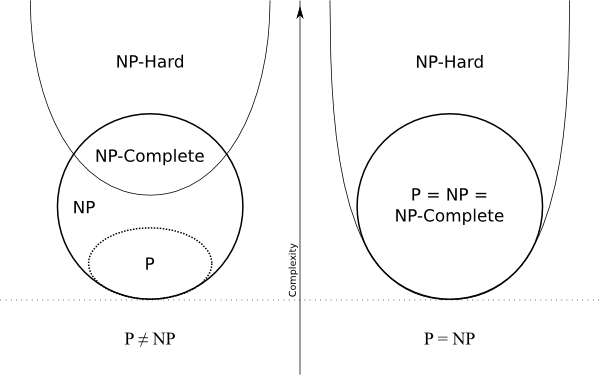
\includegraphics[scale=0.65]{images/einleitung/p_np_np-complete_np-hard.png}
\caption[Übersicht der Komplexitätsklassen ($P!=NP$ und $P=NP$)]{Übersicht der Komplexitätsklassen ($P \neq NP$ und $P=NP$) (Grafik entnommen aus \cite{pic_p_np})}
\label{fig:complexity_overview}
\end{figure}

\section{Algorithmentypen}\label{algo_types}
In diesem Abschnitt werden drei gängige Algorithmentypen erklärt, welche bei der Recherche bei der Lösung vieler Problemen zum 
Einsatz kamen. Die Aufzählung erhebt keinen Anspruch auf Vollständigkeit. Dynamic Programming oder Divide and Conquer wären 
weitere gängige Algorithmentypen, welche für das Lösen von Problemen mit hoher Laufzeitkomplexität verwendet werden \cite{vazirani_algorithm}.

\subsection{Backtracking Algorithmen}\label{backtracking_algos}
Beim Backtracking geht es darum, sich einer Lösung eines Problems schrittweise zu nähern. Bei jedem neuen Schritt wird geprüft, ob das Resultat noch eine gültige Lösung darstellt. Falls dies 
nicht der Fall ist, wird der letzte Schritt rückgängig gemacht und es wird ein anderer Weg eingeschlagen. In \cite{backtracking} wird dieses Verfahren anhand des Damenproblems aufgezeigt.

Die Laufzeit eines Backtracking Algorithmus ist Abhängig von der Eingabegrösse und der Verzweigungsrate. Im schlechtesten Fall beträgt sie
$O(z^n)$, wobei $n$ die Eingabegrösse und $z$ die Verzweigungsrate ist. Die Suche dauert oft lange, deshalb empfiehlt sich ein Backtracking 
Algorithmus nur bei kleinen Lösungsbäumen \cite{stephens2013essential}. Jedoch wird mithilfe eines Backtracking Algorithmus immer eine Lösung gefunden, falls 
eine existiert \cite{pomberger2008algorithmen}.

\subsection{Greedy Algorithmen}\label{greedy_algos}
Greedy Algorithmen liefern oft schnell eine Lösung, welche aber meist nicht optimal ist. Die Algorithmen entscheiden bei jedem Schritt, was die aktuell beste Möglichkeit ist. Da sie nicht alle 
Möglichkeiten betrachten, finden sie oft nur ein lokales Minimum bzw. Maximum \cite{mcmillan2014data}. In \autoref{fig:greedy_algo} ist in grün der Weg des Greedy Algorithmus zu sehen. 
Der Algorithmus entscheidet sich für die 12 auf der zweiten Ebene, da diese im Betrachtungsraum als beste Lösung gilt. Mit dem violetten Pfad könnte jedoch ein viel höherer Wert erzielt 
werden.

\begin{figure}[h]
\centering 
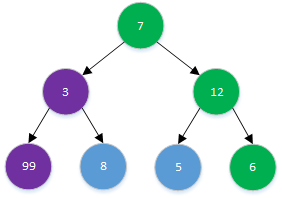
\includegraphics[scale=1]{images/einleitung/greedy_algo.png}
\caption[Suchen des profitabelsten Weg mit Hilfe eines Greedy Algorithmus]{Suchen des profitabelsten Weg mit Hilfe eines Greedy Algorithmus \selfmade{, Daten entnommen aus \cite{pic_greedy_algo}}}
\label{fig:greedy_algo}
\end{figure}

\FloatBarrier

\subsection{Evolutionäre Algorithmen}\label{ea_algos}
Evolutionäre Algorithmen nähern sich einer optimalen Lösung an. Sie basieren auf Kombinationen von Objekten und einer Fitnessfunktion zur Bewertung der einzelnen Generationen. 
Ein Ablauf eines Evolutionären Algorithmus sieht meist wie folgt aus:
\begin{enumerate}
	\item Initialisierung: Die erste Generation wird meist zufällig erzeugt
	\item Iteration durch folgende Schritte, bis zu einer bestimmten Konvergenz oder einer maximalen Anzahl an Generationen:
     	\begin{enumerate}
		\item Evaluation: Mit Hilfe der Fitnessfunktion werden die Individuen bewertet
         		\item Selektion: Auswahl von Individuen für die Rekombination
         		\item Rekombination: Erstellen einer neuen Generation durch die Kombination der ausgewählten Individuen
         		\item Mutation: Veränderung der Eigenschaften (Gene) der Nachfahren
      	\end{enumerate}
\end{enumerate}
Die Mutation und Rekombination können positive, negative oder neutrale Eigenschaften haben. Wie in der Natur überlebt der am besten Angepasste, somit wird die Lösung laufend 
besser \cite{pomberger2008algorithmen}. Evolutionäre Algorithmen sollten erst zum Einsatz kommen, wenn das Optimierungsproblem nicht effizient mit einem anderen Algorithmustyp 
gelöst werden kann. Evolutionäre Algorithmen haben oft eine höhere Laufzeit und es ist nicht garantiert, dass sie immer eine optimale Lösung liefern \cite{ea_useful}.
